\documentclass[10pt]{article}
\usepackage[margin=0.82in]{geometry}
\usepackage{booktabs,amsmath,graphicx,hyperref,xcolor}
\hypersetup{colorlinks=true,linkcolor=blue!50!black,urlcolor=blue!50!black}
\title{Progressive Retrieval Attention for llama.cpp:\\
Portable Semantic Non-Prefix Memory in the GGUF Ecosystem}
\author{Jorge Sim\~ao}
\date{September 2026}

\begin{document}
\maketitle

\begin{abstract}
llama.cpp makes quantized local inference portable across CPUs and accelerator
backends. Progressive Retrieval Attention (PRA) asks for a different form of
portability: independently addressable semantic records whose selected native
key/value (K/V) states can be reused without becoming visible prompt tokens.
We pin llama.cpp commit
\texttt{458681e1d5d4a29a1463c4732e03226cf384b997}, implement a PRA SDK adapter,
audit public slot and state APIs, and qualify selected-text execution on Apple
M4 Pro CPU and Metal backends. On a 15-example natural-QA smoke cohort,
selected prompts used 37.5--51.7\% of the full-context prompt tokens. Metal
median time to first token fell on HotpotQA (60.1 to 37.0 ms) and QASPER (58.9
to 31.0 ms), but not on 2Wiki (27.3 to 35.6 ms). A live slot checkpoint saved
13 positional tokens as 160,572 bytes and restored them in 2.327 ms. The audit
shows that this state is sequential prefix state, not detached semantic K/V.
We therefore qualify upstream llama.cpp at E0 and define, but do not claim, the
minimal native boundary required for E2.
\end{abstract}

\section{Introduction}
Local inference has two kinds of context pressure. The first is computational:
long prompts increase prefill work and K/V residency. The second is semantic:
applications need records, documents, tool outputs, and task state that do not
naturally form one immutable prefix. llama.cpp handles the first problem with
portable GGUF execution, quantization, slots, and cache controls. PRA addresses
the second by separating a logical record from the small region selected for a
particular query.

The integration question is not whether a cache can be saved. It is whether an
engine can attend to selected K/V from an independently named resource while
preserving ordinary query positions, masks, and a single normalization over
direct and memory keys. Confusing a restored conversation prefix with such
memory would produce an attractive but incorrect E2 claim.

This paper contributes: (i) a capability-honest llama.cpp SDK provider and
adapter; (ii) a pinned audit of public server and cache-state seams; (iii) live
CPU and Metal E0 qualification with frozen evidence selections; and (iv) an
explicit native-extension contract for future E2 work.

\section{PRA Contract}
For query state $q$ and selected native memory $(K_M,V_M)$, native PRA requires
one attention normalization,
\begin{equation}
 \operatorname{Attn}(q)=
 \operatorname{softmax}\!\left(
 \frac{q[K_D;K_M]^\top}{\sqrt d}+M
 \right)[V_D;V_M],
\end{equation}
where $(K_D,V_D)$ is direct sequential context and $M$ encodes the correct
causal and resource mask. Concatenating decoded memory text is E0. Restoring a
saved sequential cache is prefix reuse. Neither is native E2.

We use four evidence levels:
\begin{description}
\item[E0] selected source appears as ordinary visible text;
\item[E1] logical resource identity survives transport, but attention remains
text/prefix based;
\item[E2] the model consumes detached selected native K/V;
\item[E3] the engine scheduler owns PRA placement, prefetch, sharing, and
eviction.
\end{description}

\section{Pinned llama.cpp Audit}
The pinned source was built with CMake 4.4.3 and Ninja 1.13.2. The resulting
\texttt{llama-server} exposes OpenAI-compatible chat, explicit slots, unified KV
configuration, cache quantization, CPU execution, and Metal offload. GGUF owns
model topology and quantized weights; llama.cpp owns tensor placement, graph
execution, attention kernels, and sequential cache representation.

The public \texttt{/slots/\{id\}} save/restore API is operational only when the
server is launched with \texttt{--slot-save-path}. Its object is an engine slot:
token positions, recurrent conversational state, and ordinary cached K/V. It
does not accept an immutable resource identifier, per-layer selected intervals,
or separate direct/memory geometry. Consequently, public state APIs cannot be
used to claim E2.

\begin{figure}[t]
\centering
\fbox{\begin{minipage}{0.92\linewidth}\small
Typed PRA records $\rightarrow$ authorization and frozen selection
$\rightarrow$ \textbf{E0}: selected text in llama-server prompt.\\[2pt]
The same logical selection $\rightarrow$ resource-bound native block store
$\rightarrow$ \textbf{future E2 extension}: detached per-layer K/V
$\rightarrow$ one direct+memory attention normalization.\\[2pt]
llama.cpp independently owns GGUF loading, CPU/Metal/CUDA/Vulkan placement,
slots, scheduling, graph execution, and kernels. Slot snapshots remain on the
ordinary sequential-state path.
\end{minipage}}
\caption{Ownership and integration boundary. The upper path is measured; the
native path is a tested SDK boundary but not an upstream engine result.}
\label{fig:architecture}
\end{figure}

\section{Implementation}
\texttt{LlamaCppEngineAdapter} exposes the OpenAI-compatible path and reports E0.
An optional \texttt{LlamaCppSlotClient} derives checkpoint filenames from the
model fingerprint, tenant, session, resource URI/version, and source hash. This
prevents an application from reusing a slot solely because two visible prompts
look alike. The filename discipline improves prefix-state isolation but does
not upgrade its integration level.

Only an explicit \texttt{LlamaCppNativeExecutor} can advertise E2. It receives
the versioned \texttt{PRAWireRequest} and a \texttt{LogicalPRABlockStore}. This
small interface is the intended seam for a future llama/ggml extension that
imports selected per-layer K/V, validates model and geometry fingerprints, and
joins them to direct attention exactly once. Unit tests enforce that HTTP and
slot paths remain E0, that resource changes alter slot identity, and that only
the native executor changes the advertised capability.

\section{Experimental Method}
We used an Apple M4 Pro with 14 CPU cores, 20 GPU cores, and 48 GB unified
memory. The model was Qwen2.5-0.5B-Instruct in Q4\_K\_M GGUF. Metal used
\texttt{-ngl 99}; CPU used \texttt{-ngl 0}. Both used a 4096-token context and
four slots. The natural benchmark freezes the selected evidence before engine
execution and compares no context, E0 selected text (up to 384 source tokens),
and full context (up to 1024 source tokens). Metal covers five examples from
each of HotpotQA, QASPER, and 2WikiMultiHopQA with two repeats. CPU is a
three-example-per-dataset backend smoke test.

Quality is token F1 on short generated answers. System metrics are measured from
streaming HTTP responses. The small model, short generation cap, and small
cohort make quality directional rather than conclusive. CPU and Metal cohorts
also differ in repeat count; their absolute quality is not paired.

\section{Results}
\begin{table}[t]
\centering\small
\caption{Metal E0 qualification. Prompt ratio is selected/full. TTFT is median
milliseconds; F1 is selected/full.}
\begin{tabular}{lrrr}
\toprule Dataset & Prompt ratio & TTFT selected/full & F1 selected/full\\
\midrule
HotpotQA & 0.410 & 37.0 / 60.1 & 0.314 / 0.314\\
QASPER & 0.375 & 31.0 / 58.9 & 0.243 / 0.077\\
2Wiki & 0.517 & 35.6 / 27.3 & 0.029 / 0.129\\
\bottomrule
\end{tabular}
\label{tab:metal}
\end{table}

\begin{table}[t]
\centering\small
\caption{CPU backend smoke test. The three-case cells are calibration evidence,
not workload-scale estimates.}
\begin{tabular}{lrrr}
\toprule Dataset & Prompt ratio & TTFT selected/full & F1 selected/full\\
\midrule
HotpotQA & 0.411 & 305.5 / 530.5 & 0.103 / 0.190\\
QASPER & 0.356 & 225.7 / 534.6 & 0.070 / 0.106\\
2Wiki & 0.525 & 256.8 / 275.5 & 0.000 / 0.000\\
\bottomrule
\end{tabular}
\label{tab:cpu}
\end{table}

\begin{figure}[t]
\centering
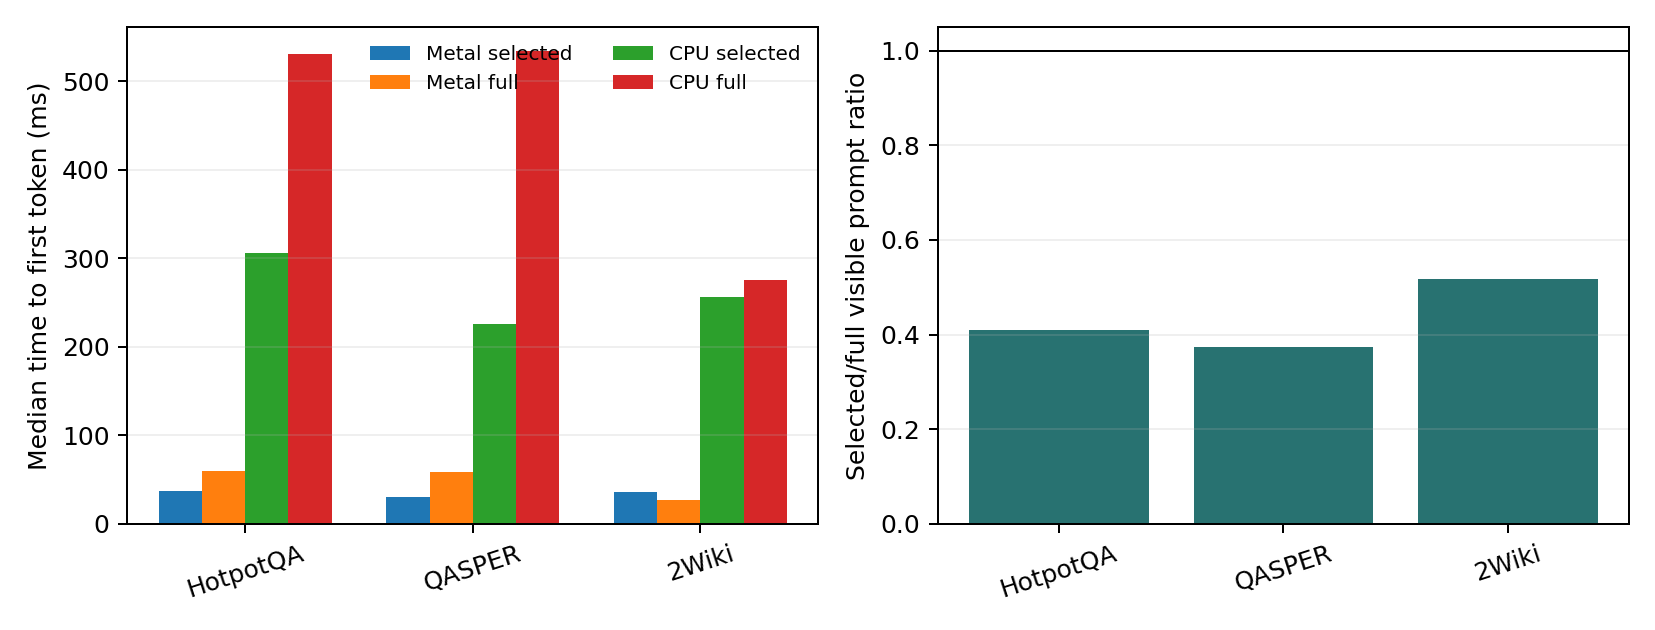
\includegraphics[width=0.97\linewidth]{figures/e0_qualification.png}
\caption{Measured E0 context-pressure qualification. Selected text reliably
reduces visible tokens; latency and quality effects remain workload dependent.}
\label{fig:e0}
\end{figure}

The robust result is input reduction, not universal quality or latency
improvement. Selected prompts occupy 35.6--52.5\% of the full prompt across the
two backend runs. Metal selected-text TTFT improves for HotpotQA and QASPER, but
2Wiki reverses direction because prefix-cache state and a short full prompt
dominate this small run. Selected evidence preserves HotpotQA F1 on Metal and
raises QASPER F1, while 2Wiki loses quality. This is consistent with an upstream
selection limitation, not evidence for or against native representation.

\subsection{Slot-state qualification}
A live slot operation saved 13 cached tokens, wrote 160,572 bytes in 0.412 ms,
and restored the same 13 tokens from 160,572 bytes in 2.327 ms. This is useful
for repeated sequential sessions. It also demonstrates why slots are not a
substitute for PRA: the saved object is much larger than a logical reference,
is position-shaped, and has no selected-resource attention contract.

\section{Capability and Stop Gate}
\begin{table}[h]
\centering\small
\caption{Qualification by backend and level at the pinned revision.}
\begin{tabular}{llll}
\toprule Backend & E0 & E2 & E3\\
\midrule
CPU & measured & not implemented & not implemented\\
Metal & measured & extension boundary only & not implemented\\
CUDA & not run here & not run & not run\\
Vulkan & not run here & not run & not run\\
\bottomrule
\end{tabular}
\end{table}

The stop gate is partially closed: E0 works, CPU and one accelerator are
measured, public state is precisely classified, and SDK isolation tests pass.
Native correctness, persistent selected K/V, physical memory accounting,
CUDA/Vulkan replication, and E3 scheduler ownership remain open.

\section{Limitations and Next Work}
The cohort is intentionally small and uses a 0.5B quantized model. We do not
measure gold-answer log probability, physical K/V sharing, concurrent tail
latency, or native E0/E2 parity. The next defensible step is the narrow native
extension in Figure~\ref{fig:architecture}, followed by geometry-matched
absent/wrong/multiple-memory controls and matched CPU, Metal, CUDA, and Vulkan
runs. Backend portability must be demonstrated independently.

\section{Conclusion}
llama.cpp already supplies a strong, portable selected-text baseline and cheap
sequential slot persistence. Its public state APIs do not provide detached
semantic K/V. PRA integration should therefore remain E0 upstream today and
move to E2 only through an explicit attention seam with resource identity,
geometry validation, isolation, and one normalization. This classification is
less dramatic than relabeling slot reuse, but it is the result another team can
reproduce and build on.

\section*{Artifact Availability}
The adapter, tests, raw JSON, figure generator, commands, and manuscript are in
branch \texttt{research/paper6-7-llamacpp}. The README records the pinned model,
backend flags, and benchmark invocation.

\begin{thebibliography}{9}
\bibitem{llamacpp} G. Gerganov et al. \emph{llama.cpp}. 2023--2026.
\url{https://github.com/ggml-org/llama.cpp}
\bibitem{gguf} llama.cpp contributors. \emph{GGUF format documentation}.
\url{https://github.com/ggml-org/ggml/blob/master/docs/gguf.md}
\bibitem{qwen25} Qwen Team. \emph{Qwen2.5 Technical Report}. 2024.
\url{https://arxiv.org/abs/2412.15115}
\end{thebibliography}
\end{document}
